\chapter{Modelos de Negócio e Proposta de Valor para Empreendimentos Tecnológicos}
\label{cap:09}
\markboth{CAPÍTULO 9: MODELOS DE NEGÓCIO}{CAPÍTULO 9: MODELOS DE NEGÓCIO}

\noindent\tagAV{Base AV3}

\begin{capObjetivos}
  Ao concluir este capítulo, você será capaz de:
  \begin{enumerate}[leftmargin=1.5em, itemsep=2pt]
    \item Explicar por que a superioridade tecnológica isolada não garante captura de valor sem um modelo de negócio coerente (\textit{Chesbrough \& Rosenbloom, 2002}).
    \item Estruturar os nove blocos do \textbf{\textit{Business Model Canvas}} (\textit{Osterwalder \& Pigneur, 2010}) e avaliar o ajuste entre Proposta de Valor e Segmento de Clientes.
    \item Integrar o processo de \textbf{\textit{Customer Development}} (\textit{Blank}) ao ciclo \textbf{\textit{Lean Startup}: Construir–Medir–Aprender} (\textit{Ries}), definindo Produtos Mínimos Viáveis (MVP).
    \item Distinguir métricas de vaidade de métricas acionáveis e calcular \textbf{CAC, LTV, razão LTV/CAC e \textit{payback} do CAC}.
  \end{enumerate}
\end{capObjetivos}

\begin{capRevisao}
  Conecte os conceitos deste capítulo com a trajetória percorrida até aqui:
  \begin{itemize}[leftmargin=1.5em, itemsep=2pt]
    \item \textbf{\textit{Effectuation} e Validação Enxuta:} o princípio da perda aceitável e a construção de alianças pré-comprometidas fornecem a base decisória para testar hipóteses antes de imobilizar capital fixo.
    \item \textbf{SOM \textit{Bottom-Up}:} o dimensionamento realista da demanda depende diretamente dos canais de distribuição e da estrutura de custos comerciais definidos no modelo de negócio.
    \item \textbf{Apropriação de Valor:} além da proteção por Propriedade Intelectual (Capítulo 8), a empresa precisa de uma arquitetura econômica que converta uso técnico em receita recorrente.
  \end{itemize}
\end{capRevisao}

\etapa{3}{Explicação Teórica, Vocabulário Prévio e Modelos}

\begin{boxSimbolo}[Vocabulário Conceitual e Símbolos do Capítulo 9]
  \begin{tabularx}{\textwidth}{@{}l >{\raggedright\arraybackslash}X@{}}
    \textbf{BMC} & \textit{Business Model Canvas}: quadro visual de nove blocos que descreve como uma organização cria, entrega e captura valor. \\
    \textbf{MVP} & \textit{Minimum Viable Product}: versão mínima de um produto capaz de completar o ciclo Construir–Medir–Aprender com o menor esforço. \\
    \textbf{CAC} & Custo de Aquisição de Cliente (despesas de marketing e vendas divididas pelos novos clientes adquiridos no período). \\
    \textbf{LTV} & \textit{Lifetime Value}: valor presente ou margem bruta acumulada gerada por um cliente durante todo o seu relacionamento com a empresa. \\
    \textbf{\textit{Churn} ($\delta$)} & Taxa mensal de cancelamento ou evasão de clientes da base ativa. \\
    \textbf{MC} & Margem de Contribuição unitária mensal por cliente ($\text{Ticket Médio} \times \text{Margem Bruta}$). \\
  \end{tabularx}
\end{boxSimbolo}

\section{Por que a Tecnologia Não Gera Valor Sozinha (Chesbrough \& Rosenbloom, 2002)}

Um equívoco recorrente em ambientes acadêmicos consiste em supor que uma invenção tecnicamente superior conquistará o mercado por mérito próprio. Ao estudar *spin-offs* tecnológicas da Xerox Corporation, Henry Chesbrough e Richard Rosenbloom (2002) indicaram que uma tecnologia possui apenas **valor econômico latente** enquanto permanece na bancada ou em relatórios técnicos. O mesmo artefato tecnológico, comercializado por meio de dois modelos de negócio distintos, produz resultados econômicos radicalmente diferentes.

Para os autores, o **modelo de negócio** atua como uma estrutura cognitiva mediadora entre o domínio técnico (insumos, parâmetros físicos, patentes) e o domínio econômico (proposta de valor para o usuário, arquitetura da cadeia de valor, estrutura de custos, margem e posição competitiva). Quando uma startup tenta vender uma tecnologia disruptiva usando o modelo de negócio legado do setor (por exemplo, exigindo alto investimento inicial em equipamento de clientes descapitalizados quando a oferta por assinatura de serviço viabilizaria a adoção), a inovação é rejeitada mesmo sendo tecnicamente superior.

\section{\textit{Business Model Canvas} (Osterwalder \& Pigneur, 2010)}

Para tornar explícita essa arquitetura de criação e captura de valor, Alexander Osterwalder e Yves Pigneur (2010) sistematizaram o **\textit{Business Model Canvas} (BMC)** em nove blocos interdependentes, divididos logicamente entre o eixo de entrega de valor (lado direito, voltado ao mercado) e o eixo de eficiência operacional (lado esquerdo, voltado à infraestrutura). No eixo de mercado, os \textbf{Segmentos de Clientes} delimitam os grupos de pessoas ou organizações com necessidades, comportamentos de compra e disposição a pagar específicas, como cooperativas agrícolas, agroindústrias médias ou secretarias municipais. Para cada segmento, a \textbf{Proposta de Valor} reúne os benefícios técnicos, econômicos ou socioambientais que resolvem uma dor relevante ou geram ganho mensurável. Essa entrega concretiza-se pelos \textbf{Canais}, que compreendem os pontos de contato físicos e digitais pelos quais a empresa comunica, vende, entrega e presta pós-venda, sendo sustentada pelo \textbf{Relacionamento com Clientes} (estratégias de aquisição, retenção e expansão via assistência técnica dedicada, autoatendimento digital ou comunidades de usuários) e monetizada pelas \textbf{Fontes de Receita}, mediante venda de ativos, assinatura recorrente, taxa de transação, licenciamento ou pagamento por desempenho.

No eixo de infraestrutura, a operação apoia-se nos \textbf{Recursos Principais} (ativos físicos, intelectuais como patentes, dados e software, humanos e financeiros indispensáveis ao modelo) e nas \textbf{Atividades-Chave}, que reúnem os processos críticos executados com excelência, como P\&D, calibração de campo, manufatura ou curadoria de dados. Como nenhuma organização jovem internaliza todas as capacidades sozinha, as \textbf{Parcerias Principais} articulam redes de fornecedores, ICTs, cooperativas e distribuidores para reduzir riscos e aportar recursos complementares, gerando ao final a \textbf{Estrutura de Custos} composta pelos gastos fixos e variáveis mais relevantes do empreendimento.

O núcleo estratégico do BMC reside no **ajuste entre Proposta de Valor e Segmento de Clientes** (*Value Proposition Fit*). Em contextos territoriais, esse ajuste exige compreender quem é o usuário técnico, quem é o decisor financeiro e quais barreiras culturais ou de infraestrutura existem no território (como conectividade intermitente no meio rural ou baixa disponibilidade de capital de giro).

\section{\textit{Customer Development}, \textit{Lean Startup} e Métricas Acionáveis}

Embora o BMC organize as hipóteses do negócio em uma única página, ele requer validação empírica contínua. Steve Blank (2005) argumentou que uma startup distingue-se de uma grande empresa consolidada por ser uma organização temporária em busca de um modelo repetível e escalável, enquanto a corporação madura executa um modelo já conhecido. Por isso, o desenvolvimento de tecnologia deve ser acompanhado pelo **\textit{Customer Development}** (Desenvolvimento de Clientes), estruturado em quatro etapas sequenciais: descoberta do cliente, validação do cliente, criação de demanda e construção da empresa.

Eric Ries (2011) operacionalizou essa lógica no movimento **\textit{Lean Startup}**, centrado no ciclo **Construir–Medir–Aprender**. Para evitar meses de desenvolvimento em sigilo sem contato com usuários, a equipe constrói um **Produto Mínimo Viável (MVP)**, que é a versão mais simples capaz de testar a hipótese central de valor com usuários reais, mede o comportamento observado e aprende se deve **perseverar** na estratégia ou **pivotar** (alterar um ou mais blocos do Canvas, como segmento, canal ou forma de cobrança).

Para que esse aprendizado seja objetivo, Ries distingue **métricas de vaidade** (números que crescem no tempo, mas falham em orientar decisões ou refletir saúde econômica, como curtidas em redes sociais, downloads brutos ou cadastros gratuitos inativos) de **métricas acionáveis**, que estabelecem relação causal entre ações operacionais e sustentabilidade financeira, como taxa de ativação, retenção por coorte, **Custo de Aquisição de Cliente (CAC)** e **Valor do Tempo de Vida do Cliente (LTV)**. A integração entre os nove blocos do BMC, o ajuste de proposta de valor ao cliente e o ciclo iterativo de validação está sintetizada na Figura~\ref{fig:09_canvas_lean}.

\begin{figure}[H]
  \centering
  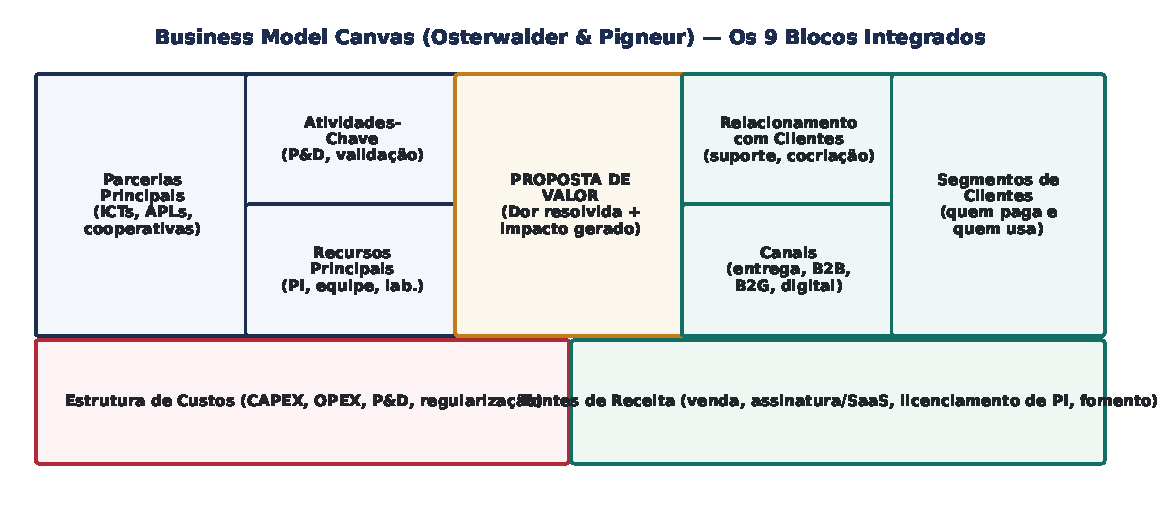
\includegraphics[width=0.95\textwidth]{figures/fig09_canvas_lean.pdf}
  \caption{Arquitetura integrada do \textit{Business Model Canvas}, ajuste Proposta de Valor–Cliente e ciclo \textit{Lean Startup} (Construir–Medir–Aprender).}
  \label{fig:09_canvas_lean}
\end{figure}

\begin{boxFormula}[Métricas Unitárias: CAC, LTV, Razão LTV/CAC e \textit{Payback} do CAC]
  \textbf{1. Custo de Aquisição de Cliente (CAC):} mede quanto custa, em média, conquistar um novo cliente pagante em determinado período:
  \[
    \text{CAC} = \frac{\text{Despesas de Marketing} + \text{Despesas de Vendas}}{\text{Número de Novos Clientes Adquiridos no Período}}.
  \]

  \textbf{2. Valor do Tempo de Vida do Cliente (LTV, \textit{Lifetime Value}):} mede a margem bruta total gerada por um cliente antes de cancelar o serviço. Sendo $\text{ARPU}$ o ticket médio mensal, $m$ a margem bruta percentual (em decimal) e $\delta$ a taxa mensal de cancelamento (\textit{churn}), o tempo médio de retenção é $\bar{T} = \frac{1}{\delta}$ meses, resultando em:
  \[
    \text{MC}_{\text{mensal}} = \text{ARPU} \times m, \qquad
    \text{LTV} = \text{MC}_{\text{mensal}} \times \bar{T} = \frac{\text{ARPU} \times m}{\delta}.
  \]

  \textbf{3. Razão LTV/CAC e Tempo de Retorno (\textit{Payback}) do CAC:}
  \[
    \text{Razão } \frac{\text{LTV}}{\text{CAC}} \ge 3{,}0 \text{ (referência saudável)}, \qquad
    \text{Payback}_{\text{CAC}} = \frac{\text{CAC}}{\text{MC}_{\text{mensal}}} \text{ (em meses)}.
  \]
  Se $\text{LTV}/\text{CAC} < 1$, a empresa destrói valor a cada novo cliente adquirido; entre $1$ e $3$, a margem para cobrir custos fixos de P\&D e estrutura é estreita; acima de $3$, o motor comercial sustenta crescimento com retorno sobre o capital investido em vendas.
\end{boxFormula}

\etapa{4}{Estudos de Caso e Exemplos Resolvidos em 7 Passos}

\begin{boxExemplo}{9.1}{Cálculo de CAC, LTV, Razão LTV/CAC e \textit{Payback} em SaaS Agrícola}
  \passoEnunciado{Uma agtech sediada em Juazeiro (BA) comercializa um software de manejo de irrigação por assinatura mensal para produtores de fruticultura.}
  \passoDados{Despesas mensais de marketing digital e feiras locais: R\$\,9.000,00. Despesas mensais com equipe de vendas técnicas (salários, comissões e deslocamento): R\$\,15.000,00. Novos clientes pagantes conquistados no mês: 20 produtores. Ticket médio mensal ($\text{ARPU}$): R\$\,450,00. Margem bruta operacional ($m$): 80\% ($0{,}80$). Taxa mensal de cancelamento (\textit{churn}, $\delta$): 4\% ($0{,}04$).}
  \passoPedido{Calcular o CAC, a margem de contribuição mensal por cliente, o tempo médio de retenção, o LTV, a razão LTV/CAC e o \textit{payback} do CAC.}
  \passoMetodo{Aplicação direta das equações unitárias de economia de assinaturas (SaaS).}
  \passoContas{
    Primeiro, calcula-se o CAC:
    \[
      \text{CAC} = \frac{9.000,00 + 15.000,00}{20} = \frac{24.000,00}{20} = \text{R\$\,1.200,00}.
    \]
    Em seguida, obtém-se a margem de contribuição mensal por cliente e o tempo médio de retenção:
    \[
      \text{MC}_{\text{mensal}} = 450,00 \times 0{,}80 = \text{R\$\,360,00/mês}, \qquad
      \bar{T} = \frac{1}{0{,}04} = 25\text{ meses}.
    \]
    Multiplicando a margem mensal pela permanência média, encontra-se o LTV:
    \[
      \text{LTV} = 360,00 \times 25 = \text{R\$\,9.000,00}.
    \]
    Por fim, avaliam-se a razão LTV/CAC e o \textit{payback} do CAC:
    \[
      \frac{\text{LTV}}{\text{CAC}} = \frac{9.000,00}{1.200,00} = 7{,}50, \qquad
      \text{Payback}_{\text{CAC}} = \frac{1.200,00}{360,00} = 3{,}33\text{ meses}.
    \]
  }
  \passoResposta{$\text{CAC} = \text{R\$\,1.200,00}$; $\text{LTV} = \text{R\$\,9.000,00}$; $\text{LTV/CAC} = 7{,}50$; \textit{payback} do CAC $= 3{,}33\text{ meses}$.}
  \passoVerificacao{Uma razão de 7{,}50 (muito acima do piso de 3{,}0) com recuperação do custo de venda em pouco mais de três meses indica forte sustentabilidade unitária para escalar a equipe comercial.}
\end{boxExemplo}

\begin{boxExemplo}{9.2}{Arquitetura do \textit{Business Model Canvas} para Rastreabilidade do Leite}
  \passoEnunciado{Uma equipe técnica propõe implantar um sistema de sensores térmicos e aplicativo de controle de qualidade do leite para cooperativas da bacia leiteira do Portal do Sertão.}
  \passoDados{Os produtores individuais têm baixa margem e resistência a mensalidades, mas os laticínios e cooperativas perdem em média 8\% do volume coletado por acidificação e pagam bônus por baixa contagem bacteriana.}
  \passoPedido{Estruturar o ajuste Proposta de Valor–Segmento de Clientes e definir os blocos críticos de Receita, Canais e Parcerias do BMC.}
  \passoMetodo{Modelagem nos nove blocos do BMC de Osterwalder e Pigneur (2010), distinguindo usuário de campo e pagador.}
  \passoContas{
    Se o modelo cobrasse dos produtores isolados, o CAC seria elevado e a conversão baixa. Ao reposicionar o \textbf{Segmento de Clientes} pagante para as cooperativas/laticínios (modelo B2B2C), a \textbf{Proposta de Valor} passa a ser a redução de descarte de leite contaminado e a elevação do preço pago por qualidade superior. Os \textbf{Canais} e \textbf{Parcerias} utilizam os próprios caminhões de coleta e técnicos de assistência rural já existentes na cooperativa, reduzindo drasticamente o custo de distribuição. A \textbf{Fonte de Receita} torna-se assinatura mensal por tanque resfriador monitorado paga pela cooperativa.
  }
  \passoResposta{Modelo B2B2C: o produtor usa o aplicativo sem custo direto; a cooperativa/laticínio paga pela assinatura por tanque monitorado em troca da redução de perdas de matéria-prima.}
  \passoVerificacao{O ajuste resolve a assimetria de capacidade de pagamento do território sem sacrificar a capilaridade de coleta de dados.}
\end{boxExemplo}

\begin{boxExemplo}{9.3}{Métricas de Vaidade vs. Métricas Acionáveis no Ciclo \textit{Lean}}
  \passoEnunciado{Um aplicativo de comercialização direta para agricultores familiares acumulou 12.000 downloads após campanha em redes sociais com gasto de R\$\,1.200,00, mas apenas 180 usuários realizaram compras recorrentes.}
  \passoDados{Investimento em mídia = R\$\,1.200,00. Downloads totais = 12.000. Compradores recorrentes antes do ajuste = 180 (taxa de conversão de download para comprador recorrente = $1{,}5\%$). Após redesenho do fluxo de cadastro (MVP 2) com o mesmo gasto de R\$\,1.200,00, os downloads foram 1.500, porém a conversão subiu para $20\%$ ($300$ compradores recorrentes).}
  \passoPedido{Identificar a métrica de vaidade e calcular o CAC efetivo por comprador recorrente antes e depois do ciclo Construir–Medir–Aprender.}
  \passoMetodo{Diferenciação entre volume bruto de exposição e custo efetivo de aquisição de usuário ativo pagante.}
  \passoContas{
    O número de downloads (12.000) é uma \textbf{métrica de vaidade}, pois mascara o abandono de $98{,}5\%$ dos usuários. Calculando o CAC efetivo por comprador recorrente:
    \[
      \text{CAC}_{\text{antes}} = \frac{1.200,00}{180} \approx \text{R\$\,6{,}67/comprador}, \qquad
      \text{CAC}_{\text{depois}} = \frac{1.200,00}{300} = \text{R\$\,4{,}00/comprador}.
    \]
    Apesar de os downloads caírem de 12.000 para 1.500, o CAC efetivo foi reduzido em $(6{,}67 - 4{,}00)/6{,}67 \approx 40{,}0\%$.
  }
  \passoResposta{Downloads constituem métrica de vaidade; o ciclo \textit{Lean} aumentou os compradores recorrentes de 180 para 300 e reduziu o CAC efetivo de R\$\,6{,}67 para R\$\,4{,}00.}
  \passoVerificacao{O exemplo ilustra por que decisões orientadas por métricas acionáveis evitam investir em divulgação antes de corrigir gargalos de ativação no MVP.}
\end{boxExemplo}

\begin{boxExemplo}{9.4}{Pivô de Modelo de Receita: Venda de Equipamento para HaaS}
  \passoEnunciado{Uma startup desenvolveu estações meteorológicas automatizadas para prefeituras e consórcios municipais. No modelo original, tentava vender cada estação por R\$\,24.000,00 à vista (CAPEX do cliente), mas esbarrava em processos licitatórios lentos e falta de manutenção local.}
  \passoDados{Custo de fabricação de cada estação: R\$\,9.000,00. Custo mensal de manutenção e conectividade: R\$\,120,00/estação. Novo modelo proposto (\textit{Hardware as a Service}, HaaS): assinatura de R\$\,920,00/mês em contrato de 36 meses, sem custo inicial de aquisição para o município.}
  \passoPedido{Calcular a margem de contribuição mensal líquida da manutenção e em quantos meses a startup recupera o custo de fabricação da estação no modelo HaaS.}
  \passoMetodo{Análise de transição CAPEX para OPEX e cálculo de \textit{payback} do equipamento.}
  \passoContas{
    Receita líquida mensal após custos recorrentes de conectividade/manutenção:
    \[
      \text{Saldo mensal por estação} = 920,00 - 120,00 = \text{R\$\,800,00/mês}.
    \]
    Tempo necessário para recuperar o custo de fabricação (R\$\,9.000,00):
    \[
      \text{Payback do hardware} = \frac{9.000,00}{800,00} = 11{,}25\text{ meses}.
    \]
    Ao longo do contrato de 36 meses, o fluxo líquido por estação após pagar o hardware será $36 \times 800,00 - 9.000,00 = 28.800,00 - 9.000,00 = \text{R\$\,19.800,00}$.
  }
  \passoResposta{O custo de fabricação é recuperado em 11{,}25 meses, gerando saldo líquido de R\$\,19.800,00 por estação ao longo de 36 meses.}
  \passoVerificacao{O pivô elimina a barreira de entrada orçamentária do cliente, mas exige da startup capital de giro para financiar os primeiros 11{,}25 meses de fabricação.}
\end{boxExemplo}

\begin{boxExemplo}{9.5}{Mediação Tecnológica e Captura de Valor (Chesbrough \& Rosenbloom)}
  \passoEnunciado{Um grupo universitário desenvolveu uma membrana filtrante cerâmica 30\% mais durável que as membranas poliméricas importadas usadas em pequenas queijarias artesanais.}
  \passoDados{A membrana importada custa R\$\,400,00 e dura 6 meses. A membrana cerâmica universitária tem custo de produção de R\$\,600,00 e dura 18 meses, mas exige um suporte de aço inox que custa R\$\,1.200,00 na primeira compra.}
  \passoPedido{Explicar por que tentar vender o conjunto inicial a R\$\,1.800,00 à vista fracassa junto às pequenas queijarias e propor uma reconfiguração de modelo de negócio.}
  \passoMetodo{Comparação de desembolso inicial vs. custo total de propriedade (TCO) e arquitetura de captura de valor.}
  \passoContas{
    Em 18 meses, a queijaria gastaria $3 \times 400,00 = \text{R\$\,1.200,00}$ com a membrana importada (desembolso parcelado de R\$\,400,00 a cada semestre). Embora a cerâmica seja tecnicamente superior, cobrar R\$\,1.800,00 à vista na entrada representa 4{,}5 vezes o desembolso semestral habitual do produtor. Se a startup mantiver a propriedade do suporte de aço inox em comodato e cobrar apenas R\$\,70,00/mês pelo serviço de filtração com reposição garantida, o gasto em 18 meses será $18 \times 70,00 = \text{R\$\,1.260,00}$ (praticamente igual ao importado), diluindo a barreira inicial e gerando receita previsível.
  }
  \passoResposta{A tecnologia fracassa no modelo de venda direta por causa da barreira de entrada de R\$\,1.800,00; o modelo de comodato com assinatura mensal destrava a adoção.}
  \passoVerificacao{O caso confirma a tese de Chesbrough e Rosenbloom (2002): a inovação está tanto no modelo de cobrança e relacionamento quanto no material cerâmico.}
\end{boxExemplo}

\etapa{5}{Armadilhas Conceituais e Erros Mais Comuns}

\begin{boxErro}[Erro 1: Preencher o \textit{Business Model Canvas} como Documento Estático]
  Muitos estudantes tratam o preenchimento dos nove quadros do BMC como o encerramento do planejamento. Na prática, um Canvas inicial é apenas um conjunto de hipóteses não verificadas; cada bloco precisa ser testado em campo e revisado à medida que entrevistas e MVPs revelam o comportamento real dos clientes.
\end{boxErro}

\begin{boxErro}[Erro 2: Calcular o LTV Sobre o Faturamento Bruto em Vez da Margem Bruta]
  Multiplicar o ticket médio pelo tempo de retenção sem aplicar a margem bruta ($m$) superestima gravemente o LTV. Em empresas com custos variáveis elevados (hardware, insumos físicos, taxas de pagamento), usar a receita bruta no numerador mascara um negócio deficitário como se tivesse boa relação LTV/CAC.
\end{boxErro}

\begin{boxErro}[Erro 3: Tratar o MVP como Produto Mal Acabado ou Defeituoso]
  Construir um MVP não significa entregar uma solução tecnicamente insegura ou inoperante ao cliente. Significa reduzir o escopo funcional ao núcleo mínimo necessário para validar a proposta de valor principal, preservando confiabilidade técnica no atributo testado.
\end{boxErro}

\begin{boxErro}[Erro 4: Subestimar Custos Comerciais no Cálculo do CAC]
  Computar apenas anúncios digitais no numerador do CAC e omitir salários de vendedores, viagens técnicas no território, comissões e tempo gasto em demonstrações distorce o indicador para baixo e compromete a projeção de capital de giro.
\end{boxErro}

\etapa{6}{Lista de Exercícios (15 Questões em 3 Níveis)}

\textbf{Nível 1, Fundamentos Conceituais (Questões 1 a 5)}

\begin{enumerate}[leftmargin=1.5em, itemsep=6pt]
  \item Explique a tese de Chesbrough e Rosenbloom (2002) sobre o papel mediador do modelo de negócio entre tecnologia e geração de valor econômico.
  \espacoResolucao[1.8cm]

  \item Liste os nove blocos do \textit{Business Model Canvas} e explique a diferença lógica entre os blocos do lado direito (valor/mercado) e os do lado esquerdo (eficiência/infraestrutura).
  \espacoResolucao[1.8cm]

  \item Diferencie as quatro etapas do \textit{Customer Development} de Steve Blank e explique por que elas antecedem a contratação de uma grande equipe de vendas.
  \espacoResolucao[1.8cm]

  \item Descreva o ciclo Construir–Medir–Aprender de Eric Ries e dê dois exemplos de métricas de vaidade e dois de métricas acionáveis para uma plataforma territorial.
  \espacoResolucao[1.8cm]

  \item Qual a diferença conceitual entre ajustar parâmetros de preço e realizar um pivô no modelo de negócio?
  \espacoResolucao[1.8cm]

  \item \textbf{(Nível 2, Aplicações Numéricas)} Uma startup investiu R\$\,18.000,00 em marketing e R\$\,27.000,00 em vendas em um trimestre, conquistando 30 novos clientes corporativos. Calcule o CAC desse período.
  \espacoResolucao[2.1cm]

  \item Um serviço de monitoramento de silos agrícolas cobra mensalidade de R\$\,600,00, apresenta margem bruta de 75\% e taxa de cancelamento (\textit{churn}) de 5\% ao mês. Calcule a margem de contribuição mensal por cliente, o tempo médio de retenção e o LTV.
  \espacoResolucao[2.2cm]

  \item Utilizando o LTV obtido no exercício anterior e considerando um $\text{CAC} = \text{R\$\,2.250,00}$, calcule a razão $\text{LTV/CAC}$ e o \textit{payback} do CAC em meses. O resultado atende ao padrão saudável do mercado?
  \espacoResolucao[2.2cm]

  \item Uma empresa tem $\text{ARPU} = \text{R\$\,200,00}$, margem bruta de 60\% e deseja manter a razão $\text{LTV/CAC} = 4{,}0$. Se o CAC atual é de R\$\,1.200,00, qual deve ser a taxa máxima mensal de \textit{churn} ($\delta$) tolerável?
  \espacoResolucao[2.3cm]

  \item Um marketplace regional gasta R\$\,4.000,00 por mês em aquisição digital. No Mês 1 obteve 2.000 cadastros gratuitos e apenas 40 vendedores ativos pagantes. No Mês 2, após simplificar o MVP, obteve 800 cadastros e 100 vendedores ativos pagantes. Calcule a variação percentual do CAC efetivo por vendedor ativo pagante.
  \espacoResolucao[2.3cm]

  \item \textbf{(Nível 3, Análise Territorial e Estratégica)} Uma cooperativa de apicultura pretende adotar um software de rastreabilidade. Estruture os nove blocos do BMC indicando explicitamente quem é o usuário de campo, quem é o pagador e quais parcerias territoriais reduzem o CAC.
  \espacoResolucao[2.3cm]

  \item Uma startup vende sensores de solo com $\text{CAC} = \text{R\$\,3.000,00}$, $\text{ARPU} = \text{R\$\,500,00}$, margem bruta $= 50\%$ e \textit{churn} $= 10\%$ ao mês. Demonstre numericamente por que escalar investimentos em vendas nessa configuração destruiria ou comprometeria o capital da empresa e proponha duas alavancas corretivas.
  \espacoResolucao[2.4cm]

  \item Explique como o uso de cooperativas, sindicatos rurais ou associações comerciais como **Canais** e **Parcerias Principais** no BMC altera simultaneamente o CAC e o tempo de retenção (LTV) em territórios interioranos.
  \espacoResolucao[2.2cm]

  \item Uma empresa vende um software agrícola com contrato anual pago à vista de R\$\,4.800,00 (equivalente a R\$\,400,00/mês) e margem bruta de 85\%. Se o \textit{churn} anualizado corresponder a uma permanência média de 30 meses e o CAC for de R\$\,2.040,00, calcule o LTV, a razão LTV/CAC e explique a vantagem financeira da cobrança anual antecipada sobre o fluxo de caixa.
  \espacoResolucao[2.4cm]

  \item Desenhe um protocolo de MVP de baixo custo (sem programação pesada) para validar a disposição a pagar de pequenas agroindústrias baianas por um serviço de certificação energética e rastreabilidade ambiental.
  \espacoResolucao[2.3cm]
\end{enumerate}

\etapa{7}{Questões Autorais Estilo Pós-Graduação / Concursos de CT\&I}

\begin{enumerate}[leftmargin=1.5em, itemsep=6pt]
  \item \textbf{(Estilo ANPAD / Estratégia e Inovação)} Sobre o ciclo \textit{Lean Startup} e a economia unitária de modelos de negócio, analise as afirmações:
  I. O LTV deve ser calculado considerando a margem bruta gerada pelo cliente ao longo do seu tempo de retenção, e não apenas o faturamento bruto, sob pena de superestimar a viabilidade de aquisição.
  II. Um elevado volume de downloads gratuitos ou seguidores em redes sociais caracteriza uma métrica acionável suficiente para validar o \textit{Product-Market Fit}.
  III. Em mercados territoriais pulverizados, parcerias institucionais com cooperativas e associações podem reduzir o CAC ao concentrar múltiplos usuários em um único canal de venda.
  Assinale a alternativa correta:
  \begin{alternativas}
    \item Apenas I está correta.
    \item Apenas II está correta.
    \item Apenas I e III estão corretas.
    \item Apenas II e III estão corretas.
    \item I, II e III estão corretas.
  \end{alternativas}
  \espacoResolucao[1.5cm]

  \item \textbf{(Estilo Concurso Analista de Projetos / Gestão)} Uma empresa de serviços digitais para gestão hídrica possui ticket médio mensal de R\$\,500,00, margem bruta de 70\%, \textit{churn} mensal de 2{,}5\% e CAC de R\$\,3.500,00. Assinale a alternativa que apresenta corretamente o LTV, a razão LTV/CAC e o \textit{payback} do CAC:
  \begin{alternativas}
    \item $\text{LTV} = \text{R\$\,14.000,00}$; $\text{LTV/CAC} = 4{,}0$; $\text{Payback} = 10{,}0\text{ meses}$.
    \item $\text{LTV} = \text{R\$\,20.000,00}$; $\text{LTV/CAC} = 5{,}7$; $\text{Payback} = 7{,}0\text{ meses}$.
    \item $\text{LTV} = \text{R\$\,14.000,00}$; $\text{LTV/CAC} = 4{,}0$; $\text{Payback} = 7{,}0\text{ meses}$.
    \item $\text{LTV} = \text{R\$\,10.500,00}$; $\text{LTV/CAC} = 3{,}0$; $\text{Payback} = 10{,}0\text{ meses}$.
    \item $\text{LTV} = \text{R\$\,17.500,00}$; $\text{LTV/CAC} = 5{,}0$; $\text{Payback} = 10{,}0\text{ meses}$.
  \end{alternativas}
  \espacoResolucao[1.6cm]

  \item \textbf{(Estilo Discursiva, PPGPT)} Um laboratório universitário desenvolveu um método eficiente para transformar resíduos de cacau em embalagem biodegradável, porém nenhuma indústria regional adquiriu o processo quando ofertado via venda direta de patente. Com base em Chesbrough \& Rosenbloom (2002) e Osterwalder \& Pigneur (2010), explique por que a excelência técnica falhou em gerar adoção e proponha uma reformulação de modelo de negócio.
  \espacoResolucao[2.4cm]
\end{enumerate}

\begin{boxDica}[Contraponto Crítico e Prática Territorial (AV3)]
  No Projeto Final (AV3), apresente o \textit{Business Model Canvas} completo do seu empreendimento ou arranjo territorial, mas não se limite a preencher os nove quadros: explicite qual é a hipótese mais arriscada do Canvas, qual MVP foi ou será usado para testá-la e calcule explicitamente o CAC e o LTV esperados.
\end{boxDica}

\clearpage
\etapa{8}{Gabarito Integralmente Comentado (Exercícios 1 a 18)}

\begin{boxGabarito}[Resolução Completa dos Exercícios da Etapa 6 (1 a 15) e Etapa 7 (16 a 18)]
  \begin{enumerate}[leftmargin=1.5em, itemsep=4pt]
    \item \textbf{Resposta:} Segundo Chesbrough e Rosenbloom (2002), a tecnologia possui apenas valor latente; o modelo de negócio funciona como mediador cognitivo e econômico que define proposta de valor, segmento, cadeia produtiva e mecanismo de captura de receita.
    \item \textbf{Resposta:} Os 9 blocos são: Segmentos de Clientes, Proposta de Valor, Canais, Relacionamento, Fontes de Receita (eixo de valor/mercado, lado direito); Recursos Principais, Atividades-Chave, Parcerias Principais e Estrutura de Custos (eixo de eficiência/infraestrutura, lado esquerdo).
    \item \textbf{Resposta:} Descoberta do cliente, Validação do cliente, Criação de demanda e Construção da empresa. As duas primeiras etapas verificam se há dor real e disposição a pagar antes de investir pesado em força comercial.
    \item \textbf{Resposta:} Construir (MVP) $\to$ Medir (comportamento real) $\to$ Aprender (perseverar ou pivotar). Vaidade: curtidas e downloads brutos. Acionáveis: taxa de ativação pagante, retenção mensal e CAC.
    \item \textbf{Resposta:} Ajustar preço é uma otimização tática dentro da mesma hipótese de negócio; pivotar é mudar estruturalmente um ou mais pilares do modelo (segmento, proposta de valor, canal ou forma de monetização).
    \item \textbf{Resposta:} $\text{CAC} = (18.000 + 27.000) / 30 = 45.000 / 30 = \text{R\$\,1.500,00}$.
    \item \textbf{Resposta:} $\text{MC}_{\text{mensal}} = 600 \times 0{,}75 = \text{R\$\,450,00/mês}$. Retenção média $= 1 / 0{,}05 = 20\text{ meses}$. $\text{LTV} = 450 \times 20 = \text{R\$\,9.000,00}$.
    \item \textbf{Resposta:} $\text{LTV/CAC} = 9.000 / 2.250 = 4{,}0$. $\text{Payback}_{\text{CAC}} = 2.250 / 450 = 5{,}0\text{ meses}$. Sim, atende ao padrão saudável ($\text{LTV/CAC} \ge 3{,}0$).
    \item \textbf{Resposta:} $\text{MC}_{\text{mensal}} = 200 \times 0{,}60 = \text{R\$\,120,00}$. Para $\text{LTV/CAC} = 4{,}0$, exige-se $\text{LTV} = 4 \times 1.200 = \text{R\$\,4.800,00}$. Como $\text{LTV} = \text{MC}_{\text{mensal}} / \delta$, tem-se $\delta = 120 / 4.800 = 0{,}025 = 2{,}5\%$ ao mês.
    \item \textbf{Resposta:} $\text{CAC}_{\text{M1}} = 4.000 / 40 = \text{R\$\,100,00}$. $\text{CAC}_{\text{M2}} = 4.000 / 100 = \text{R\$\,40,00}$. Redução de $(100 - 40)/100 = 60\%$.
    \item \textbf{Resposta:} Usuário: apicultor cooperado; Pagador: cooperativa ou entreposto exportador; Parcerias: cooperativas, SENAR/SEBRAE e ICTs; Canais: técnicos de campo da cooperativa, reduzindo drasticamente o CAC unitário.
    \item \textbf{Resposta:} $\text{MC}_{\text{mensal}} = 500 \times 0{,}50 = \text{R\$\,250,00}$. Retenção $= 1 / 0{,}10 = 10\text{ meses}$. $\text{LTV} = 250 \times 10 = \text{R\$\,2.500,00}$. Como $\text{CAC} = \text{R\$\,3.000,00}$, $\text{LTV/CAC} = 2.500 / 3.000 \approx 0{,}83 < 1{,}0$ e o \textit{payback} ($3.000 / 250 = 12\text{ meses}$) supera a permanência média (10 meses), destruindo R\$\,500,00 por cliente. Alavancas: reduzir o CAC via vendas em grupo (cooperativas) e reduzir o \textit{churn} com suporte pós-venda.
    \item \textbf{Resposta:} Vender via cooperativas dilui o esforço de prospecção em dezenas de produtores por contrato (reduzindo o CAC) e ancora o uso da solução na rotina coletiva (reduzindo o \textit{churn} e elevando o LTV).
    \item \textbf{Resposta:} $\text{MC}_{\text{mensal}} = 400 \times 0{,}85 = \text{R\$\,340,00}$. $\text{LTV} = 340 \times 30 = \text{R\$\,10.200,00}$. $\text{LTV/CAC} = 10.200 / 2.040 = 5{,}0$. A cobrança anual antecipada (R\$\,4.800,00 no ato) cobre imediatamente o CAC de R\$\,2.040,00, financiando o crescimento sem depender de capital de giro externo.
    \item \textbf{Resposta:} MVP tipo *concierge* ou página de pré-reserva: apresentar um dossiê demonstrativo a 10 agroindústrias com simulação personalizada de economia energética e solicitar carta de intenção ou pagamento simbólico de diagnóstico piloto antes de desenvolver a plataforma automatizada.
    \item \textbf{Questão 16 (Etapa 7), Gabarito: (C).} II é falsa porque downloads gratuitos e seguidores são métricas de vaidade.
    \item \textbf{Questão 17 (Etapa 7), Gabarito: (A).} $\text{MC}_{\text{mensal}} = 500 \times 0{,}70 = \text{R\$\,350,00}$; Retenção $= 1 / 0{,}025 = 40\text{ meses}$; $\text{LTV} = 350 \times 40 = \text{R\$\,14.000,00}$; $\text{LTV/CAC} = 14.000 / 3.500 = 4{,}0$; $\text{Payback} = 3.500 / 350 = 10{,}0\text{ meses}$.
    \item \textbf{Questão 18 (Etapa 7), Espelho Discursivo:} Deve explicar que a venda direta de patente transfere todo o risco tecnológico e de escala para indústrias locais que não têm P\&D interna. A reformulação propõe ofertar a embalagem pronta (via parceria com convertedor local ou produção sob contrato) ou licenciamento escalonado por volume com validação piloto compartilhada.
  \end{enumerate}
\end{boxGabarito}

\begin{boxResumo}
  \begin{itemize}[leftmargin=1.4em, itemsep=2pt]
    \item O modelo de negócio traduz potencial técnico em captura econômica de valor.
    \item O \textit{Business Model Canvas} integra mercado (lado direito) e operação (lado esquerdo) a partir do ajuste Proposta de Valor–Segmento de Clientes.
    \item O ciclo Construir–Medir–Aprender via MVPs substitui suposições por métricas acionáveis: $\text{LTV/CAC} \ge 3{,}0$ e \textit{payback} do CAC inferior ao tempo de retenção.
  \end{itemize}
\end{boxResumo}

\begin{boxTeste}
  \begin{enumerate}[leftmargin=1.5em, itemsep=4pt]
    \item (\V/\F) Segundo Chesbrough e Rosenbloom (2002), uma tecnologia superior captura valor automaticamente no mercado, independentemente do modelo de negócio adotado.
    \item (\V/\F) No cálculo do LTV, deve-se multiplicar a receita mensal pela margem bruta antes de dividir pela taxa mensal de \textit{churn}.
    \item (\V/\F) Se $\text{CAC} = \text{R\$\,1.000,00}$, $\text{ARPU} = \text{R\$\,250,00}$, margem bruta $= 80\%$ e \textit{churn} $= 5\%$ ao mês, então $\text{LTV} = \text{R\$\,4.000,00}$ e $\text{LTV/CAC} = 4{,}0$.
    \item (\V/\F) O total de curtidas e visualizações em redes sociais é exemplo clássico de métrica acionável para comprovar validação de modelo de negócio.
  \end{enumerate}
  \begin{boxGabarito}[Respostas do Checkpoint: Capítulo 9]
    \textbf{1: \F} (O modelo de negócio é o mediador indispensável). \quad \textbf{2: \V}. \quad \textbf{3: \V} ($\text{MC} = 200$; Retenção $= 20$; $\text{LTV} = 4.000$; $\text{LTV/CAC} = 4{,}0$). \quad \textbf{4: \F} (Trata-se de métrica de vaidade).
  \end{boxGabarito}
\end{boxTeste}
